% Graphic for TeX using PGF
% Title: /home/indenml/code/bachelor_thesis/content/figures/language_spec-erm-dimension.dia
% Creator: Dia v0.97.3
% CreationDate: Mon Aug  8 11:29:07 2016
% For: indenml
% \usepackage{tikz}
% The following commands are not supported in PSTricks at present
% We define them conditionally, so when they are implemented,
% this pgf file will use them.
\ifx\du\undefined
  \newlength{\du}
\fi
\setlength{\du}{15\unitlength}
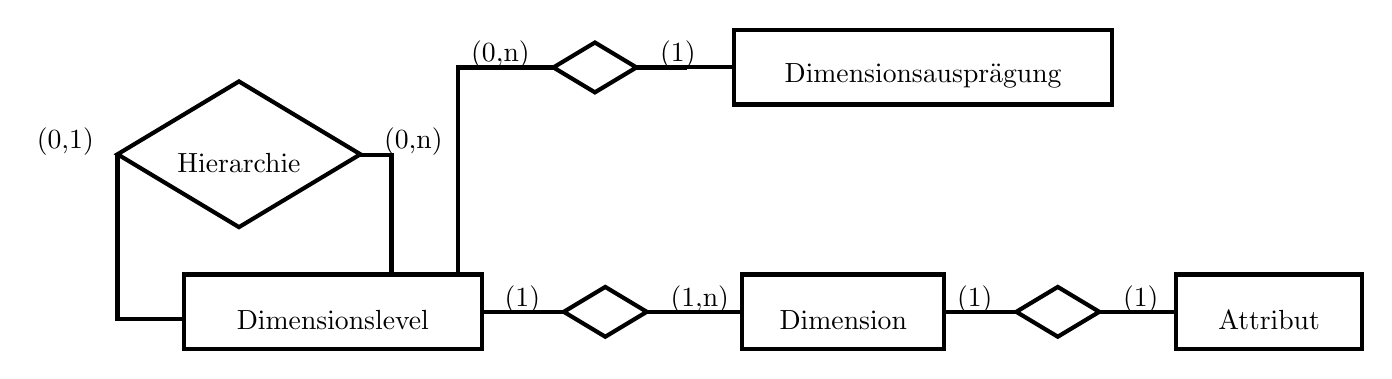
\begin{tikzpicture}
\pgftransformxscale{1.000000}
\pgftransformyscale{-1.000000}
\definecolor{dialinecolor}{rgb}{0.000000, 0.000000, 0.000000}
\pgfsetstrokecolor{dialinecolor}
\definecolor{dialinecolor}{rgb}{1.000000, 1.000000, 1.000000}
\pgfsetfillcolor{dialinecolor}
\definecolor{dialinecolor}{rgb}{1.000000, 1.000000, 1.000000}
\pgfsetfillcolor{dialinecolor}
\fill (26.650000\du,14.200000\du)--(26.650000\du,16.000000\du)--(31.515000\du,16.000000\du)--(31.515000\du,14.200000\du)--cycle;
\pgfsetlinewidth{0.100000\du}
\pgfsetdash{}{0pt}
\pgfsetmiterjoin
\definecolor{dialinecolor}{rgb}{0.000000, 0.000000, 0.000000}
\pgfsetstrokecolor{dialinecolor}
\draw (26.650000\du,14.200000\du)--(26.650000\du,16.000000\du)--(31.515000\du,16.000000\du)--(31.515000\du,14.200000\du)--cycle;
% setfont left to latex
\definecolor{dialinecolor}{rgb}{0.000000, 0.000000, 0.000000}
\pgfsetstrokecolor{dialinecolor}
\node at (29.082500\du,15.300000\du){Dimension};
\definecolor{dialinecolor}{rgb}{1.000000, 1.000000, 1.000000}
\pgfsetfillcolor{dialinecolor}
\fill (13.200000\du,14.200000\du)--(13.200000\du,16.000000\du)--(20.375000\du,16.000000\du)--(20.375000\du,14.200000\du)--cycle;
\pgfsetlinewidth{0.100000\du}
\pgfsetdash{}{0pt}
\pgfsetmiterjoin
\definecolor{dialinecolor}{rgb}{0.000000, 0.000000, 0.000000}
\pgfsetstrokecolor{dialinecolor}
\draw (13.200000\du,14.200000\du)--(13.200000\du,16.000000\du)--(20.375000\du,16.000000\du)--(20.375000\du,14.200000\du)--cycle;
% setfont left to latex
\definecolor{dialinecolor}{rgb}{0.000000, 0.000000, 0.000000}
\pgfsetstrokecolor{dialinecolor}
\node at (16.787500\du,15.300000\du){Dimensionslevel};
\definecolor{dialinecolor}{rgb}{1.000000, 1.000000, 1.000000}
\pgfsetfillcolor{dialinecolor}
\fill (37.100000\du,14.200000\du)--(37.100000\du,16.000000\du)--(41.580000\du,16.000000\du)--(41.580000\du,14.200000\du)--cycle;
\pgfsetlinewidth{0.100000\du}
\pgfsetdash{}{0pt}
\pgfsetmiterjoin
\definecolor{dialinecolor}{rgb}{0.000000, 0.000000, 0.000000}
\pgfsetstrokecolor{dialinecolor}
\draw (37.100000\du,14.200000\du)--(37.100000\du,16.000000\du)--(41.580000\du,16.000000\du)--(41.580000\du,14.200000\du)--cycle;
% setfont left to latex
\definecolor{dialinecolor}{rgb}{0.000000, 0.000000, 0.000000}
\pgfsetstrokecolor{dialinecolor}
\node at (39.340000\du,15.300000\du){Attribut};
\definecolor{dialinecolor}{rgb}{1.000000, 1.000000, 1.000000}
\pgfsetfillcolor{dialinecolor}
\fill (11.600000\du,11.305000\du)--(14.525000\du,9.550000\du)--(17.450000\du,11.305000\du)--(14.525000\du,13.060000\du)--cycle;
\pgfsetlinewidth{0.100000\du}
\pgfsetdash{}{0pt}
\pgfsetmiterjoin
\definecolor{dialinecolor}{rgb}{0.000000, 0.000000, 0.000000}
\pgfsetstrokecolor{dialinecolor}
\draw (11.600000\du,11.305000\du)--(14.525000\du,9.550000\du)--(17.450000\du,11.305000\du)--(14.525000\du,13.060000\du)--cycle;
% setfont left to latex
\definecolor{dialinecolor}{rgb}{0.000000, 0.000000, 0.000000}
\pgfsetstrokecolor{dialinecolor}
\node[anchor=east] at (11.300000\du,11.005000\du){(0,1)};
\definecolor{dialinecolor}{rgb}{0.000000, 0.000000, 0.000000}
\pgfsetstrokecolor{dialinecolor}
\node[anchor=west] at (17.750000\du,11.005000\du){(0,n)};
\definecolor{dialinecolor}{rgb}{0.000000, 0.000000, 0.000000}
\pgfsetstrokecolor{dialinecolor}
\node at (14.525000\du,11.505000\du){Hierarchie};
\pgfsetlinewidth{0.100000\du}
\pgfsetdash{}{0pt}
\pgfsetmiterjoin
\pgfsetbuttcap
\definecolor{dialinecolor}{rgb}{0.000000, 0.000000, 0.000000}
\pgfsetstrokecolor{dialinecolor}
\draw (13.200000\du,15.100000\du)--(13.200000\du,15.269600\du)--(11.600000\du,15.269600\du)--(11.600000\du,11.305000\du);
\pgfsetlinewidth{0.100000\du}
\pgfsetdash{}{0pt}
\pgfsetmiterjoin
\pgfsetbuttcap
\definecolor{dialinecolor}{rgb}{0.000000, 0.000000, 0.000000}
\pgfsetstrokecolor{dialinecolor}
\draw (16.787500\du,14.200000\du)--(18.200000\du,14.200000\du)--(18.200000\du,11.319600\du)--(17.450000\du,11.319600\du)--(17.450000\du,11.305000\du);
\definecolor{dialinecolor}{rgb}{1.000000, 1.000000, 1.000000}
\pgfsetfillcolor{dialinecolor}
\fill (22.350000\du,15.100000\du)--(23.350000\du,14.500000\du)--(24.350000\du,15.100000\du)--(23.350000\du,15.700000\du)--cycle;
\pgfsetlinewidth{0.100000\du}
\pgfsetdash{}{0pt}
\pgfsetmiterjoin
\definecolor{dialinecolor}{rgb}{0.000000, 0.000000, 0.000000}
\pgfsetstrokecolor{dialinecolor}
\draw (22.350000\du,15.100000\du)--(23.350000\du,14.500000\du)--(24.350000\du,15.100000\du)--(23.350000\du,15.700000\du)--cycle;
% setfont left to latex
\definecolor{dialinecolor}{rgb}{0.000000, 0.000000, 0.000000}
\pgfsetstrokecolor{dialinecolor}
\node[anchor=east] at (22.050000\du,14.800000\du){(1) };
\definecolor{dialinecolor}{rgb}{0.000000, 0.000000, 0.000000}
\pgfsetstrokecolor{dialinecolor}
\node[anchor=west] at (24.650000\du,14.800000\du){(1,n) };
\definecolor{dialinecolor}{rgb}{0.000000, 0.000000, 0.000000}
\pgfsetstrokecolor{dialinecolor}
\node at (23.350000\du,15.300000\du){};
\pgfsetlinewidth{0.100000\du}
\pgfsetdash{}{0pt}
\pgfsetmiterjoin
\pgfsetbuttcap
\definecolor{dialinecolor}{rgb}{0.000000, 0.000000, 0.000000}
\pgfsetstrokecolor{dialinecolor}
\draw (26.650000\du,15.100000\du)--(26.600000\du,15.100000\du)--(24.400000\du,15.100000\du)--(24.350000\du,15.100000\du);
\pgfsetlinewidth{0.100000\du}
\pgfsetdash{}{0pt}
\pgfsetmiterjoin
\pgfsetbuttcap
\definecolor{dialinecolor}{rgb}{0.000000, 0.000000, 0.000000}
\pgfsetstrokecolor{dialinecolor}
\draw (22.350000\du,15.100000\du)--(22.200000\du,15.100000\du)--(22.200000\du,15.100000\du)--(20.375000\du,15.100000\du);
\definecolor{dialinecolor}{rgb}{1.000000, 1.000000, 1.000000}
\pgfsetfillcolor{dialinecolor}
\fill (33.250000\du,15.100000\du)--(34.250000\du,14.500000\du)--(35.250000\du,15.100000\du)--(34.250000\du,15.700000\du)--cycle;
\pgfsetlinewidth{0.100000\du}
\pgfsetdash{}{0pt}
\pgfsetmiterjoin
\definecolor{dialinecolor}{rgb}{0.000000, 0.000000, 0.000000}
\pgfsetstrokecolor{dialinecolor}
\draw (33.250000\du,15.100000\du)--(34.250000\du,14.500000\du)--(35.250000\du,15.100000\du)--(34.250000\du,15.700000\du)--cycle;
% setfont left to latex
\definecolor{dialinecolor}{rgb}{0.000000, 0.000000, 0.000000}
\pgfsetstrokecolor{dialinecolor}
\node[anchor=east] at (32.950000\du,14.800000\du){(1)};
\definecolor{dialinecolor}{rgb}{0.000000, 0.000000, 0.000000}
\pgfsetstrokecolor{dialinecolor}
\node[anchor=west] at (35.550000\du,14.800000\du){(1)};
\definecolor{dialinecolor}{rgb}{0.000000, 0.000000, 0.000000}
\pgfsetstrokecolor{dialinecolor}
\node at (34.250000\du,15.300000\du){};
\definecolor{dialinecolor}{rgb}{1.000000, 1.000000, 1.000000}
\pgfsetfillcolor{dialinecolor}
\fill (22.100000\du,9.212500\du)--(23.100000\du,8.612500\du)--(24.100000\du,9.212500\du)--(23.100000\du,9.812500\du)--cycle;
\pgfsetlinewidth{0.100000\du}
\pgfsetdash{}{0pt}
\pgfsetmiterjoin
\definecolor{dialinecolor}{rgb}{0.000000, 0.000000, 0.000000}
\pgfsetstrokecolor{dialinecolor}
\draw (22.100000\du,9.212500\du)--(23.100000\du,8.612500\du)--(24.100000\du,9.212500\du)--(23.100000\du,9.812500\du)--cycle;
% setfont left to latex
\definecolor{dialinecolor}{rgb}{0.000000, 0.000000, 0.000000}
\pgfsetstrokecolor{dialinecolor}
\node[anchor=east] at (21.800000\du,8.912500\du){(0,n)};
\definecolor{dialinecolor}{rgb}{0.000000, 0.000000, 0.000000}
\pgfsetstrokecolor{dialinecolor}
\node[anchor=west] at (24.400000\du,8.912500\du){(1)};
\definecolor{dialinecolor}{rgb}{0.000000, 0.000000, 0.000000}
\pgfsetstrokecolor{dialinecolor}
\node at (23.100000\du,9.412500\du){};
\pgfsetlinewidth{0.100000\du}
\pgfsetdash{}{0pt}
\pgfsetmiterjoin
\pgfsetbuttcap
\definecolor{dialinecolor}{rgb}{0.000000, 0.000000, 0.000000}
\pgfsetstrokecolor{dialinecolor}
\draw (33.250000\du,15.100000\du)--(33.200000\du,15.100000\du)--(31.565000\du,15.100000\du)--(31.515000\du,15.100000\du);
\pgfsetlinewidth{0.100000\du}
\pgfsetdash{}{0pt}
\pgfsetmiterjoin
\pgfsetbuttcap
\definecolor{dialinecolor}{rgb}{0.000000, 0.000000, 0.000000}
\pgfsetstrokecolor{dialinecolor}
\draw (35.250000\du,15.100000\du)--(35.300000\du,15.100000\du)--(37.050000\du,15.100000\du)--(37.100000\du,15.100000\du);
\pgfsetlinewidth{0.100000\du}
\pgfsetdash{}{0pt}
\pgfsetmiterjoin
\pgfsetbuttcap
\definecolor{dialinecolor}{rgb}{0.000000, 0.000000, 0.000000}
\pgfsetstrokecolor{dialinecolor}
\draw (20.375000\du,14.200000\du)--(19.800000\du,14.200000\du)--(19.800000\du,9.212500\du)--(22.100000\du,9.212500\du);
\pgfsetlinewidth{0.100000\du}
\pgfsetdash{}{0pt}
\pgfsetmiterjoin
\pgfsetbuttcap
\definecolor{dialinecolor}{rgb}{0.000000, 0.000000, 0.000000}
\pgfsetstrokecolor{dialinecolor}
\draw (24.100000\du,9.212500\du)--(25.277500\du,9.212500\du)--(25.277500\du,9.205000\du)--(26.455000\du,9.205000\du);
\definecolor{dialinecolor}{rgb}{1.000000, 1.000000, 1.000000}
\pgfsetfillcolor{dialinecolor}
\fill (26.455000\du,8.305000\du)--(26.455000\du,10.105000\du)--(35.555000\du,10.105000\du)--(35.555000\du,8.305000\du)--cycle;
\pgfsetlinewidth{0.100000\du}
\pgfsetdash{}{0pt}
\pgfsetmiterjoin
\definecolor{dialinecolor}{rgb}{0.000000, 0.000000, 0.000000}
\pgfsetstrokecolor{dialinecolor}
\draw (26.455000\du,8.305000\du)--(26.455000\du,10.105000\du)--(35.555000\du,10.105000\du)--(35.555000\du,8.305000\du)--cycle;
% setfont left to latex
\definecolor{dialinecolor}{rgb}{0.000000, 0.000000, 0.000000}
\pgfsetstrokecolor{dialinecolor}
\node at (31.005000\du,9.405000\du){Dimensionsausprägung};
\end{tikzpicture}
